\documentclass{standalone}
\usepackage{tikz}
\usetikzlibrary{patterns, positioning}
\usepackage[sfdefault]{ClearSans} %% option 'sfdefault' activates Clear Sans as the default text font
\usepackage[T1]{fontenc}

\begin{document}
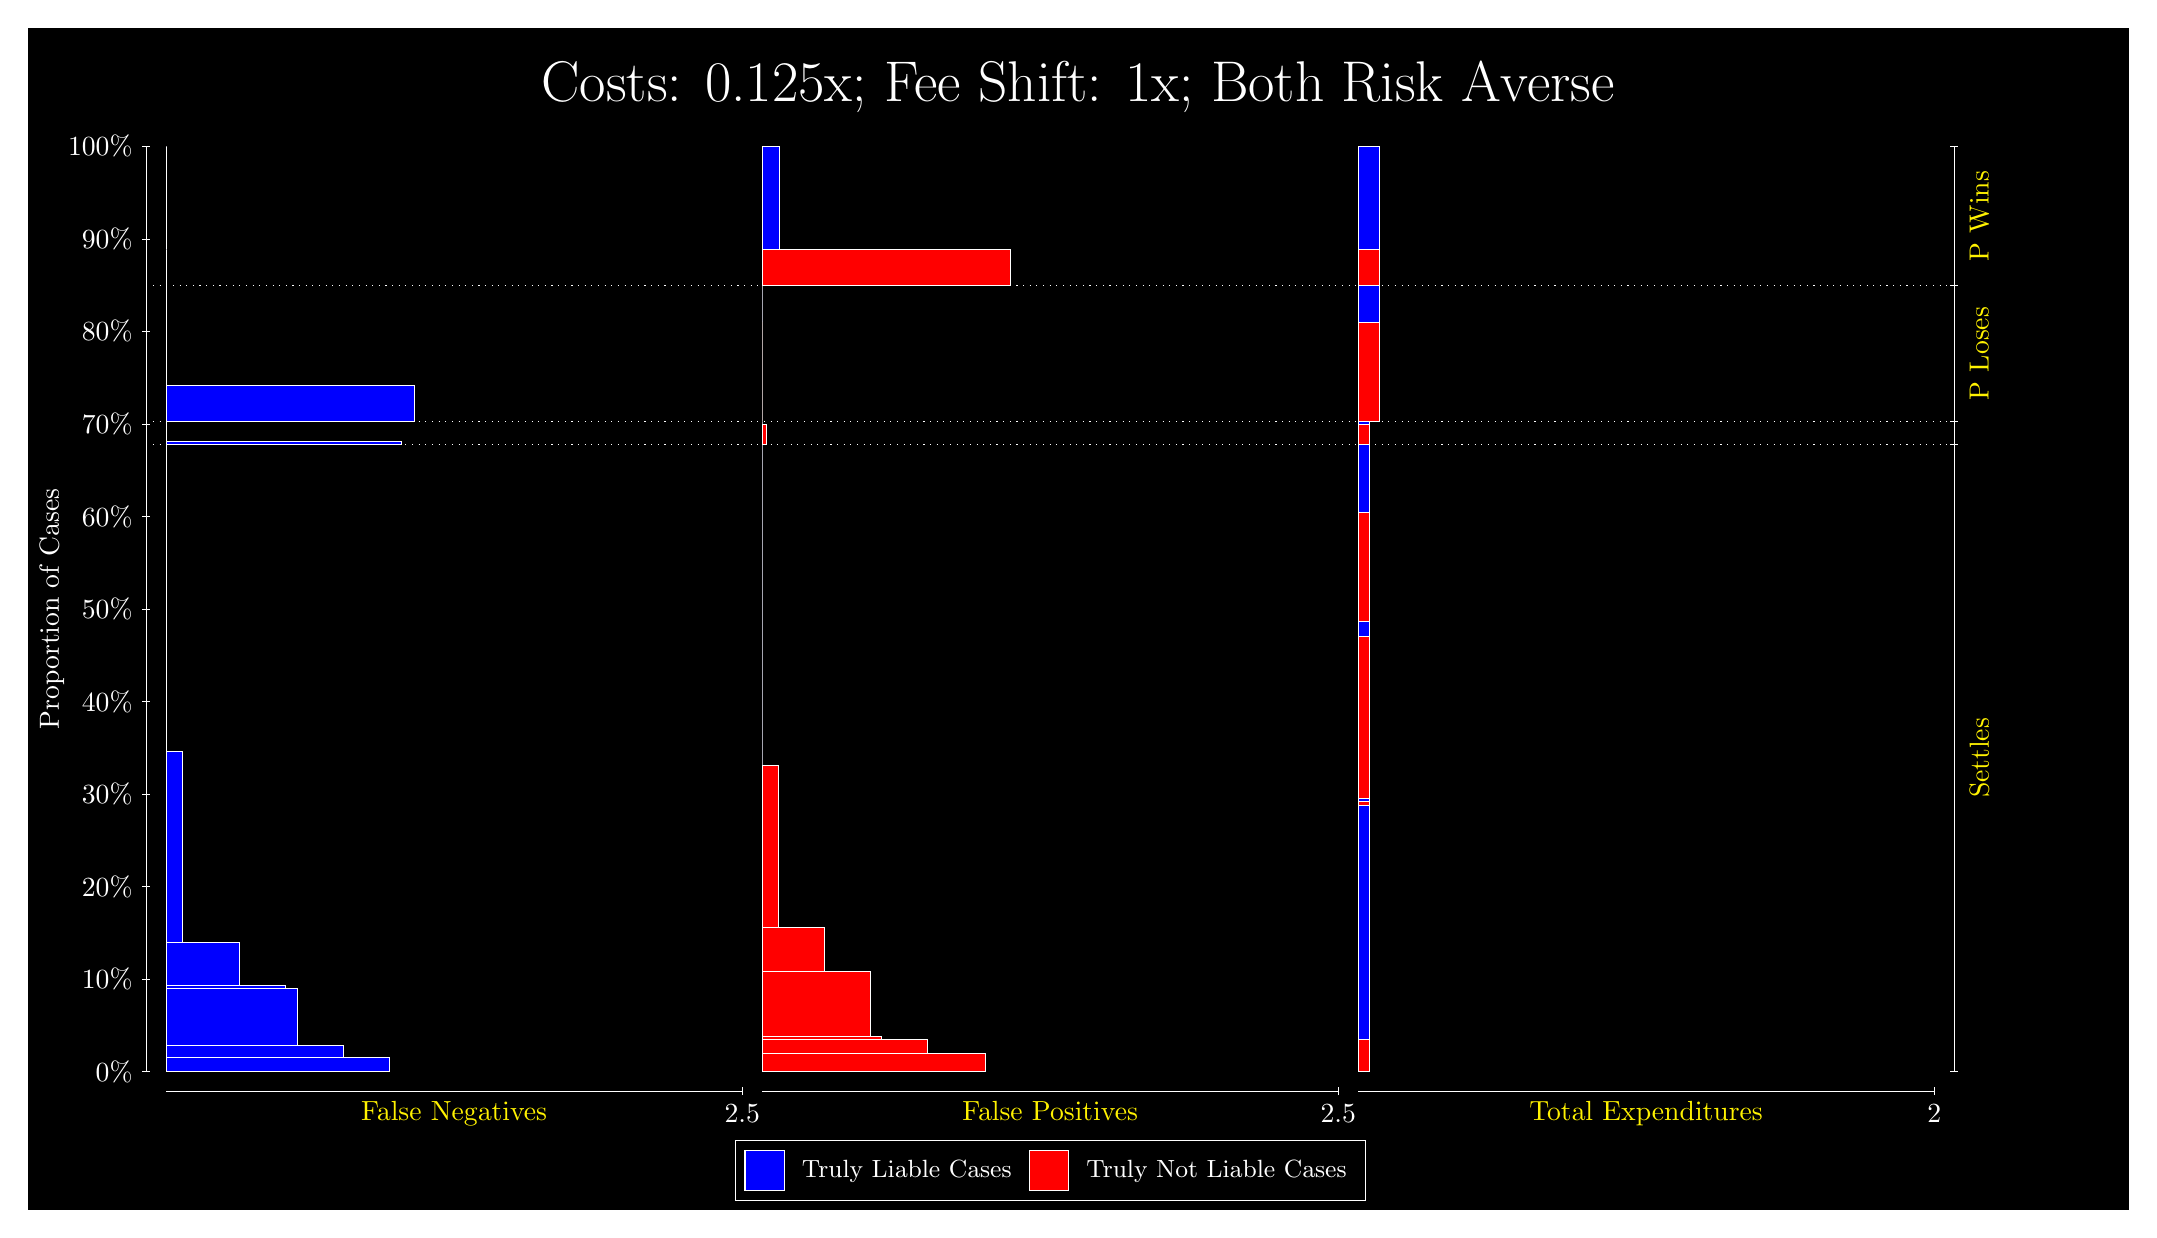
\begin{tikzpicture}
\draw[fill=black] (0,0) rectangle (26.667,15);
\draw[text=white] (0,13.5) rectangle (26.667,15) node[midway] {\huge Costs: 0.125x; Fee Shift: 1x; Both Risk Averse};
\draw[white, very thin] (1.5,1.75) -- (1.5,13.5);
\node[rotate=90, text=white, anchor=center] at (0.3, 7.625) {Proportion of Cases};
\draw[white, very thin] (1.45,1.75) -- (1.55,1.75);
\node[text=white, anchor=east] at (1.45, 1.75) {0\%};
\draw[white, very thin] (1.45,2.925) -- (1.55,2.925);
\node[text=white, anchor=east] at (1.45, 2.925) {10\%};
\draw[white, very thin] (1.45,4.1) -- (1.55,4.1);
\node[text=white, anchor=east] at (1.45, 4.1) {20\%};
\draw[white, very thin] (1.45,5.275) -- (1.55,5.275);
\node[text=white, anchor=east] at (1.45, 5.275) {30\%};
\draw[white, very thin] (1.45,6.45) -- (1.55,6.45);
\node[text=white, anchor=east] at (1.45, 6.45) {40\%};
\draw[white, very thin] (1.45,7.625) -- (1.55,7.625);
\node[text=white, anchor=east] at (1.45, 7.625) {50\%};
\draw[white, very thin] (1.45,8.8) -- (1.55,8.8);
\node[text=white, anchor=east] at (1.45, 8.8) {60\%};
\draw[white, very thin] (1.45,9.975) -- (1.55,9.975);
\node[text=white, anchor=east] at (1.45, 9.975) {70\%};
\draw[white, very thin] (1.45,11.15) -- (1.55,11.15);
\node[text=white, anchor=east] at (1.45, 11.15) {80\%};
\draw[white, very thin] (1.45,12.325) -- (1.55,12.325);
\node[text=white, anchor=east] at (1.45, 12.325) {90\%};
\draw[white, very thin] (1.45,13.5) -- (1.55,13.5);
\node[text=white, anchor=east] at (1.45, 13.5) {100\%};

\draw[white, very thin] (24.457,1.75) -- (24.457,13.5);
\draw[white, very thin] (24.407,1.75) -- (24.507,1.75);
\node[anchor=west] at (24.407, 1.75) {};
\draw[white, very thin] (24.407,9.7174) -- (24.507,9.7174);
\node[anchor=west] at (24.407, 9.7174) {};
\draw[white, very thin] (24.407,10.008) -- (24.507,10.008);
\node[anchor=west] at (24.407, 10.008) {};
\draw[white, very thin] (24.407,11.731) -- (24.507,11.731);
\node[anchor=west] at (24.407, 11.731) {};
\draw[white, very thin] (24.407,13.5) -- (24.507,13.5);
\node[anchor=west] at (24.407, 13.5) {};

\draw[white, very thin, fill=blue] (1.75,1.75) rectangle (4.5861,1.9328);
\draw[white, very thin, fill=blue] (1.75,1.9328) rectangle (4.0006,2.0782);
\draw[white, very thin, fill=blue] (1.75,2.0782) rectangle (3.415,2.8034);
\draw[white, very thin, fill=blue] (1.75,2.8034) rectangle (3.2687,2.8435);
\draw[white, very thin, fill=blue] (1.75,2.8435) rectangle (2.6832,3.3886);
\draw[white, very thin, fill=blue] (1.75,3.3886) rectangle (1.9513,5.8235);
\draw[white, very thin, fill=red] (1.75,5.8235) rectangle (1.75,9.7174);
\draw[white, very thin, fill=blue] (1.75,9.7174) rectangle (4.7324,9.7493);
\draw[white, very thin, fill=red] (1.75,9.7493) rectangle (1.75,10.008);
\draw[white, very thin, fill=blue] (1.75,10.008) rectangle (4.8971,10.469);
\draw[white, very thin, fill=red] (1.75,10.469) rectangle (1.75,11.731);
\draw[white, very thin, fill=red] (1.75,11.731) rectangle (1.75,12.192);
\draw[white, very thin, fill=blue] (1.75,12.192) rectangle (1.75,13.5);
\draw[white, very thin, fill=red] (9.3189,1.75) rectangle (12.155,1.9819);
\draw[white, very thin, fill=red] (9.3189,1.9819) rectangle (11.423,2.1539);
\draw[white, very thin, fill=red] (9.3189,2.1539) rectangle (10.838,2.1965);
\draw[white, very thin, fill=red] (9.3189,2.1965) rectangle (10.691,3.0247);
\draw[white, very thin, fill=red] (9.3189,3.0247) rectangle (10.106,3.5795);
\draw[white, very thin, fill=red] (9.3189,3.5795) rectangle (9.5201,5.6438);
\draw[white, very thin, fill=blue] (9.3189,5.6438) rectangle (9.3189,9.7174);
\draw[white, very thin, fill=red] (9.3189,9.7174) rectangle (9.3738,9.9757);
\draw[white, very thin, fill=blue] (9.3189,9.9757) rectangle (9.3189,10.008);
\draw[white, very thin, fill=red] (9.3189,10.008) rectangle (9.3189,11.269);
\draw[white, very thin, fill=blue] (9.3189,11.269) rectangle (9.3189,11.731);
\draw[white, very thin, fill=red] (9.3189,11.731) rectangle (12.466,12.192);
\draw[white, very thin, fill=blue] (9.3189,12.192) rectangle (9.5384,13.5);
\draw[white, very thin, fill=red] (16.888,1.75) rectangle (17.025,2.1539);
\draw[white, very thin, fill=blue] (16.888,2.1539) rectangle (17.025,5.1339);
\draw[white, very thin, fill=red] (16.888,5.1339) rectangle (17.025,5.1765);
\draw[white, very thin, fill=blue] (16.888,5.1765) rectangle (17.025,5.2166);
\draw[white, very thin, fill=red] (16.888,5.2166) rectangle (17.025,7.281);
\draw[white, very thin, fill=blue] (16.888,7.281) rectangle (17.025,7.4638);
\draw[white, very thin, fill=red] (16.888,7.4638) rectangle (17.025,8.8468);
\draw[white, very thin, fill=blue] (16.888,8.8468) rectangle (17.025,9.7174);
\draw[white, very thin, fill=red] (16.888,9.7174) rectangle (17.025,9.9757);
\draw[white, very thin, fill=blue] (16.888,9.9757) rectangle (17.025,10.008);
\draw[white, very thin, fill=red] (16.888,10.008) rectangle (17.162,11.269);
\draw[white, very thin, fill=blue] (16.888,11.269) rectangle (17.162,11.731);
\draw[white, very thin, fill=red] (16.888,11.731) rectangle (17.162,12.192);
\draw[white, very thin, fill=blue] (16.888,12.192) rectangle (17.162,13.5);
\draw[white, dotted] (1.5,9.7174) -- (24.457,9.7174);
\draw[white, dotted] (1.5,10.008) -- (24.457,10.008);
\draw[white, dotted] (1.5,11.731) -- (24.457,11.731);
\draw[white, very thin] (1.75,1.5) -- (9.0689,1.5);
\node[text=yellow, anchor=north] at (5.4094, 1.5) {False Negatives};
\draw[white, very thin] (9.0689,1.45) -- (9.0689,1.55);
\node[text=white, anchor=north] at (9.0689, 1.45) {2.5};

\draw[white, very thin] (9.3189,1.5) -- (16.638,1.5);
\node[text=yellow, anchor=north] at (12.978, 1.5) {False Positives};
\draw[white, very thin] (16.638,1.45) -- (16.638,1.55);
\node[text=white, anchor=north] at (16.638, 1.45) {2.5};

\draw[white, very thin] (16.888,1.5) -- (24.207,1.5);
\node[text=yellow, anchor=north] at (20.547, 1.5) {Total Expenditures};
\draw[white, very thin] (24.207,1.45) -- (24.207,1.55);
\node[text=white, anchor=north] at (24.207, 1.45) {2};

\node[text=yellow, centered, rotate=90] at (24.777, 5.7337) {Settles};

\node[text=yellow, centered, rotate=90] at (24.777, 10.869) {P Loses};
\node[text=yellow, centered, rotate=90] at (24.777, 12.615) {P Wins};

\draw (12.978300999999998,1.5) node[draw=none] (baseCoordinate) {};
\begin{scope}[align=center]
        \matrix[scale=0.5, draw=white, below=0.5cm of baseCoordinate, nodes={draw}, column sep=0.1cm]{
            \node[rectangle, draw, minimum width=0.5cm, minimum height=0.5cm, fill=blue] {}; &
            \node[draw=none, font=\small, text=white] (B) {Truly Liable Cases}; &
            \node[rectangle, draw, minimum width=0.5cm, minimum height=0.5cm, fill=red] {}; &
            \node[draw=none, font=\small, text=white] (B) {Truly Not Liable Cases}; \\
            };
\end{scope}

\end{tikzpicture}
\end{document}